\documentclass[11pt,a4paper,oneside]{report}
\usepackage{amsmath,amssymb,calc,ifthen}
\usepackage{float}
%\usepackage{cancel}
\usepackage[table,usenames,dvipsnames]{xcolor} % for coloured cells in tables
\usepackage{tikz}
% Allows us to click on links and references!
\usepackage{hyperref}
\usepackage{url}
\hypersetup{
colorlinks,
citecolor=blue,
filecolor=black,
linkcolor=blue,
urlcolor=black
}
% Nice package for plotting graphs
% See excellent guide:
% http://www.tug.org/TUGboat/tb31-1/tb97wright-pgfplots.pdf
\usetikzlibrary{plotmarks,shapes}
\usepackage{amsmath,graphicx}
\usepackage{epstopdf}
\usepackage{caption}
\usepackage{subcaption}
% highlight - useful for TODOs and similar
\usepackage{color}
\newcommand{\hilight}[1]{\colorbox{yellow}{#1}}
\newcommand\ci{\perp\!\!\!\perp} % perpendicular sign
\newcommand*\rfrac[2]{{}^{#1}\!/_{#2}} % diagonal fraction
\newcommand\SLASH{\char`\\}
\usepackage{listings}
% margin size
\usepackage[margin=0.65in]{geometry}

\usepackage{titlesec} % reduce spacing after subsections

% \titlespacing\subsection{0pt}{4pt plus 4pt minus 2pt}{4pt plus 2pt minus 2pt}

\usepackage{multicol}

\tikzstyle{state}=[circle,thick,draw=black, align=center, minimum size=2.1cm,
inner sep=0]
\tikzstyle{vertex}=[circle,thick,draw=black]
\tikzstyle{terminal}=[rectangle,thick,draw=black]
\tikzstyle{edge} = [draw,thick]
\tikzstyle{lo} = [edge,dotted]
\tikzstyle{hi} = [edge]
\tikzstyle{trans} = [edge,->]
\definecolor{mygreen}{rgb}{0,0.6,0}
\definecolor{mygray}{rgb}{0.5,0.5,0.5}
\definecolor{mymauve}{rgb}{0.58,0,0.82}
\DeclareMathOperator*{\argmin}{arg\,min}
\DeclareMathOperator*{\argmax}{arg\,max}
\lstset{ %
backgroundcolor=\color{white}, % choose the background color; you must add
%\usepackage{color} or \usepackage{xcolor}
basicstyle=\footnotesize, % the size of the fonts that are used for the
%code
breakatwhitespace=false, % sets if automatic breaks should only happen
%at whitespace
breaklines=true, % sets automatic line breaking
captionpos=b, % sets the caption-position to bottom
commentstyle=\color{mygreen}, % comment style
deletekeywords={...}, % if you want to delete keywords from the
%given language
escapeinside={\%*}{*)}, % if you want to add LaTeX within your code
extendedchars=true, % lets you use non-ASCII characters; for
%8-bits encodings only, does not work with UTF-8
frame=single, % adds a frame around the code
keepspaces=true, % keeps spaces in text, useful for keeping
%indentation of code (possibly needs columns=flexible)
keywordstyle=\color{blue}, % keyword style
language=Octave, % the language of the code
morekeywords={*,...}, % if you want to add more keywords to the set
numbers=left, % where to put the line-numbers; possible
%values are (none, left, right)
numbersep=5pt, % how far the line-numbers are from the code
numberstyle=\tiny\color{mygray}, % the style that is used for the line-numbers
rulecolor=\color{black}, % if not set, the frame-color may be changed
%on line-breaks within not-black text (e.g. comments (green here))
showspaces=false, % show spaces everywhere adding particular
%underscores; it overrides 'showstringspaces'
showstringspaces=false, % underline spaces within strings only
showtabs=false, % show tabs within strings adding particular
%underscores
stepnumber=2, % the step between two line-numbers. If it's
%1, each line will be numbered
stringstyle=\color{mymauve}, % string literal style
tabsize=2, % sets default tabsize to 2 spaces
title=\lstname % show the filename of files included with
%\lstinputlisting; also try caption instead of title
}
\title{Computational Modelling for Biomedical Imaging - Individual Report}
\author{
Razvan Valentin Marinescu\\
Student Number: 14060166\\
\texttt{razvan.marinescu.14@ucl.ac.uk}
}



\begin{document}
% \belowdisplayskip=12pt plus 3pt minus 9pt
% \belowdisplayshortskip=7pt plus 3pt minus 4pt

\begin{titlepage}
\begin{center}

% Upper part of the page. The '~' is needed because \\
% only works if a paragraph has started.

\includegraphics[width=0.2\textwidth]{ucl-logo2}~\\[1cm]

\textsc{\LARGE University College London}\\[1.5cm]

\newcommand{\HRule}{\rule{\linewidth}{0.5mm}}

% Title
\HRule \\[0.4cm]
{ \Large Information Processing in Medical Imaging - Coursework Report \\[0.4cm] }

\HRule \\[1.5cm]

% Author and supervisor
\begin{minipage}{0.4\textwidth}
% \begin{flushleft} \large
\centering
\emph{Author:}\\
R\u{a}zvan Valentin \textsc{Marinescu}\\
\href{razvan.marinescu.14@ucl.ac.uk}{razvan.marinescu.14@ucl.ac.uk}\\
% \end{flushleft}
\end{minipage}


\vfill

\vfill
\vfill

EPSRC Centre for Doctoral Training in Medical Imaging\\ University College London

\vfill

% Bottom of the page
{\large \today}

\end{center}
\end{titlepage}


%\maketitle{}



% \rowcolors{2}{gray!25}{white}

\section*{Task I - Full brain segmentation}

\subsection*{Proposed pipeline}

Segmentation propagation (\texttt{p1reg.py}) has been performed on the extra 5 AD and 5 controls, both baseline and followup images, using the tutorial instructions from the CMIC TIG website. This meant that we needed to propagate segmentations for 20 different images, and since we had 10 source templates available, this meant 200 propagations. A discussion about how I optimised this process and chose the parameters for the functions is given at the end of this section. Figure \ref{fig:init} shows the difference between the reference image and the floating (template) image, and we can clearly see that they are not aligned at all. Therefore, we first perform an affine transformation (\texttt{reg\_aladin}) and plot the difference images in figure \ref{fig:affine}. After this linear transformation, the brains align better, with the overall boundaries fitting well. Afterwards, we perform a non-linear registration using a free-form deformation (\texttt{reg\_f3d}) and using the affine transformation as a starting position (see figure \ref{fig:f3d}). Here, there is even more improvement in the registration of certain microstructures such as the ventricles and lobes, as well as in the overall brain boundary. We then use this transformation to propagate the segmentation of the template image into the space of the reference image. This process is repeated for all 10 template images and then a simple majority voting is used to find the final segmentation. Figure \ref{fig:segOverlay} shows that the propagated segmentation matches well with the underlying T1 scan. We then run this pipeline for all the AD and control subjects, both baseline and followup scans.

\begin{figure}[H]
        \centering
        \begin{subfigure}[b]{0.3\textwidth}
                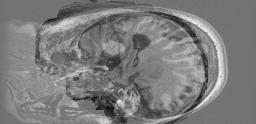
\includegraphics[width=\textwidth, height=0.8\textwidth, angle=90]{figures/diff/t1Init_x.jpg}
        \end{subfigure}%
         %add desired spacing between images, e. g. ~, \quad, \qquad, \hfill etc.
          %(or a blank line to force the subfigure onto a new line)
        \begin{subfigure}[b]{0.3\textwidth}
                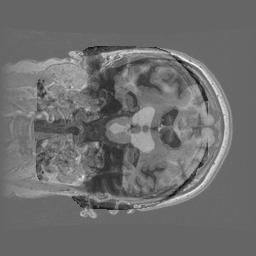
\includegraphics[width=\textwidth, angle=90]{figures/diff/t1Init_y.jpg}
        \end{subfigure}
        ~~~~ %add desired spacing between images, e. g. ~, \quad, \qquad, \hfill etc.
          %(or a blank line to force the subfigure onto a new line)
        \begin{subfigure}[b]{0.3\textwidth}
                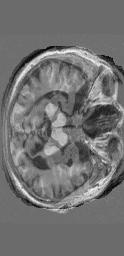
\includegraphics[width=\textwidth, height=\textwidth, trim=0 20 0 20, clip=true, angle=90 ]{figures/diff/t1Init_z.jpg}
        \end{subfigure}
        \caption{Difference image after no transformation}\label{fig:init}
\end{figure}

\begin{figure}[H]
        \centering
        \begin{subfigure}[b]{0.3\textwidth}
                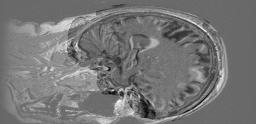
\includegraphics[width=\textwidth, height=0.8\textwidth, angle=90]{figures/diff/t1Aff_x.jpg}
        \end{subfigure}%
         %add desired spacing between images, e. g. ~, \quad, \qquad, \hfill etc.
          %(or a blank line to force the subfigure onto a new line)
        \begin{subfigure}[b]{0.3\textwidth}
                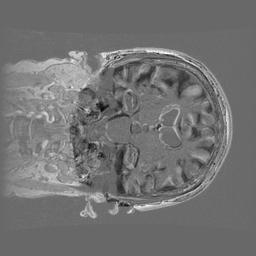
\includegraphics[width=\textwidth, angle=90]{figures/diff/t1Aff_y.jpg}
        \end{subfigure}
        ~~~~ %add desired spacing between images, e. g. ~, \quad, \qquad, \hfill etc.
          %(or a blank line to force the subfigure onto a new line)
        \begin{subfigure}[b]{0.3\textwidth}
                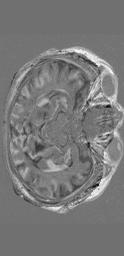
\includegraphics[width=\textwidth, height=\textwidth, trim=0 20 0 20, clip=true, angle=90 ]{figures/diff/t1Aff_z.jpg}
        \end{subfigure}
        \caption{Difference image after affine transformation}\label{fig:affine}
\end{figure}

\begin{figure}[H]
        \centering
        \begin{subfigure}[b]{0.3\textwidth}
                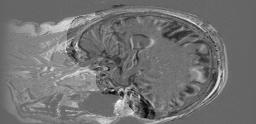
\includegraphics[width=\textwidth, height=0.8\textwidth, angle=90]{figures/diff/t1Nonlin_x.jpg}
        \end{subfigure}%
         %add desired spacing between images, e. g. ~, \quad, \qquad, \hfill etc.
          %(or a blank line to force the subfigure onto a new line)
        \begin{subfigure}[b]{0.3\textwidth}
                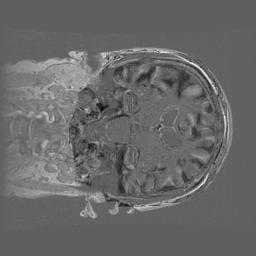
\includegraphics[width=\textwidth, angle=90]{figures/diff/t1Nonlin_y.jpg}
        \end{subfigure}
        ~~~~ %add desired spacing between images, e. g. ~, \quad, \qquad, \hfill etc.
          %(or a blank line to force the subfigure onto a new line)
        \begin{subfigure}[b]{0.3\textwidth}
                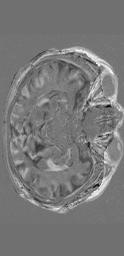
\includegraphics[width=\textwidth, height=\textwidth, trim=0 20 0 20, clip=true, angle=90 ]{figures/diff/t1Nonlin_z.jpg}
        \end{subfigure}
        \caption{Difference image after affine and nonlinear transformation using the free-form deformation algorithm}\label{fig:f3d}
\end{figure}

\begin{figure}[H]
        \centering
        \begin{subfigure}[b]{0.3\textwidth}
                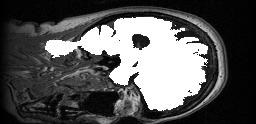
\includegraphics[width=\textwidth, height=0.8\textwidth, angle=90]{figures/diff/t1Seg_x.jpg}
        \end{subfigure}%
         %add desired spacing between images, e. g. ~, \quad, \qquad, \hfill etc.
          %(or a blank line to force the subfigure onto a new line)
        \begin{subfigure}[b]{0.3\textwidth}
                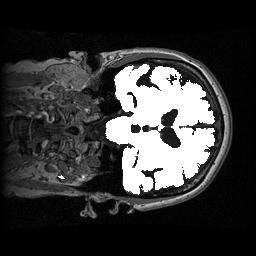
\includegraphics[width=\textwidth, angle=90]{figures/diff/t1Seg_y.jpg}
        \end{subfigure}
        ~~~~ %add desired spacing between images, e. g. ~, \quad, \qquad, \hfill etc.
          %(or a blank line to force the subfigure onto a new line)
        \begin{subfigure}[b]{0.3\textwidth}
                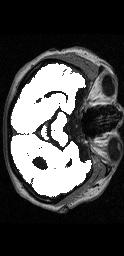
\includegraphics[width=\textwidth, height=\textwidth, trim=0 20 0 20, clip=true, angle=90 ]{figures/diff/t1Seg_z.jpg}
        \end{subfigure}
        \caption{T1 image and corresponding segmentation after label fusion with a simple majority voting}\label{fig:segOverlay}
\end{figure}


\subsection*{Parameters}

As each propagation took around 1.5 minutes on an Intel(R) Xeon(R) CPU @ 3.60GHz, a careful balance between computation time and accuracy had to be obtained. In order to find out which set of parameters to choose, we computed the dice score on the template database using a leave one out approach. More precisely, for each template image, we propagated the segmentations from the 9 other templates, performed label fusion and computed the dice score. This pipeline was then repeated for the other template images and for other sets of parameters. For the nonlinear deformation \texttt{reg\_f3d} function, we tried 4 values for the number of levels: [2,3,4,5] and 4 values for the number of iterations: [50, 150, 200, 300]. In figure \ref{fig:dice} we plotted the dice score for all these combinations, while in figure \ref{fig:time} we calculated wall-clock time taken to perform the computation on the PC.
We notice that the dice score and computation times are not much affected by the number of levels used (notice the small range of the Y-axis in the dice score plot). However, as the number of iterations increases, we see slight improvements in the dice scores but also increases in the computation time. Finally, we decided to use 4 levels and 200 iterations, in order to keep a balance between computation time and dice scores.

\begin{figure}
 \centering
 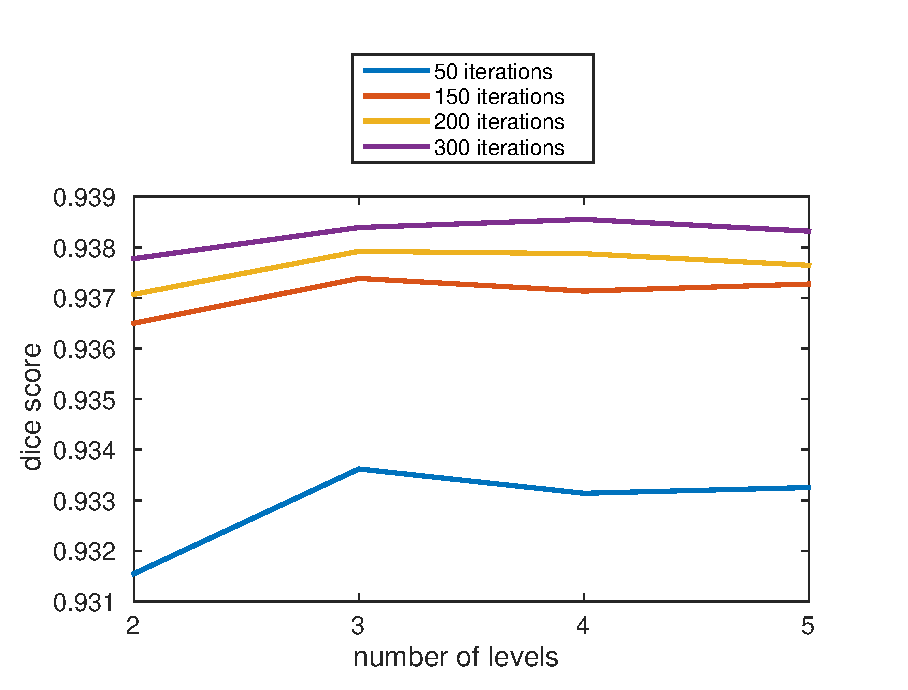
\includegraphics[scale=0.8]{figures/dice_params.eps}
 \caption{Dice scores for different number of levels and iterations.}
 \label{fig:dice}
\end{figure}

\begin{figure}
 \centering
 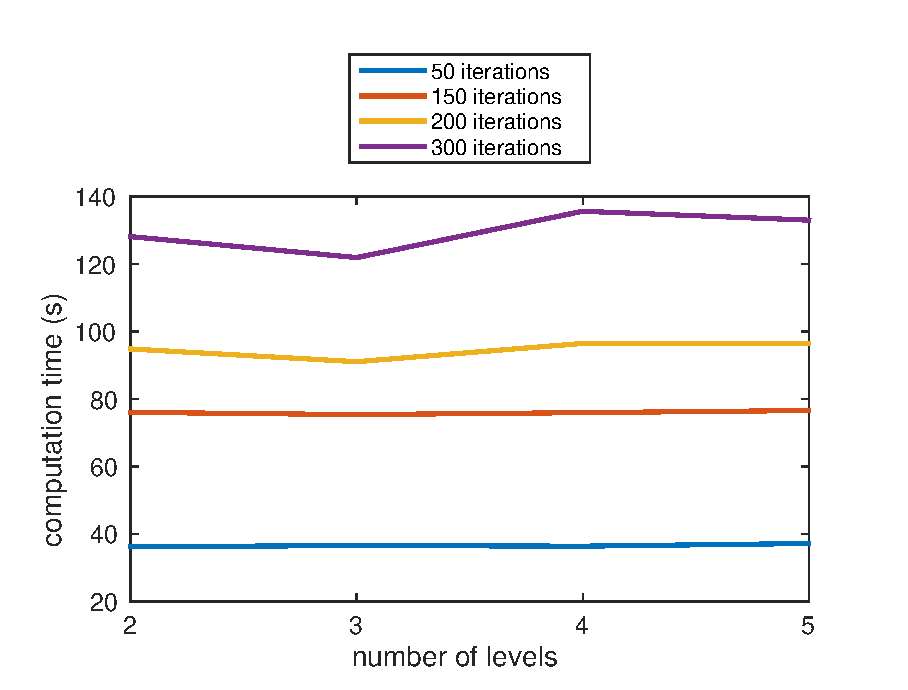
\includegraphics[scale=0.8]{figures/time_params.eps}
 \caption{Computation time for different number of levels and iterations.}
 \label{fig:time}
\end{figure}




\section*{Task II - Atrophy measurement}

In order to compute the BSI, we first co-registered the baseline and followup images to midspace and also propagated the segmentations to midspace. Afterwards, the BSI has been computed using the method described in Leung et al. \cite{leung2010robust}. First, the baseline and followup images have been aligned using the 9DOF affine registration. Then, the union and intersection regions of the images is computed. The union is dilated once, while the intersection is eroded once using a structure that looks like a 3x3x3 sphere. The brain boundary shift region is then given by the XOR of the dilated union and eroded intersection. Figure \ref{fig:bsiBoundary}  shows the boundary region for the first AD patient. The intensity of both images is then normalised by dividing by the mean intensity inside the intersect region. Finally, the BSI is computed using a manually chosen intensity window of [0.45,0.65] recommended by Freeborough and Fox, 1997. \cite{freeborough1997boundary}. Apart from the BSI, we have also computed the segmentation volume difference.

Figures \ref{fig:bsi_plot} and \ref{fig:volumeDiff_plot} show the BSI and segmentation volume difference respectively, for all age-matched AD and control subject pairs. We can clearly notice that the BSI is much better at separating the age-matched AD and controls, which is an indication that BSI can better measure atrophy in the brain. Only for AD-control pair 15 do we get that the BSI is lower in the AD subject than in the age-matched control, suggesting this pair might be an outlier. On the other hand, the segmentation volume difference cannot easily discriminate between AD and controls (figure \ref{fig:volumeDiff_plot}).

\begin{figure}[H]
        \centering
        \begin{subfigure}[b]{0.3\textwidth}
                
\includegraphics[width=\textwidth, height=0.8\textwidth, angle=90]{figures/diff/bsiBoundary_x.jpg}
        \end{subfigure}%
         %add desired spacing between images, e. g. ~, \quad, \qquad, \hfill etc.
          %(or a blank line to force the subfigure onto a new line)
        \begin{subfigure}[b]{0.3\textwidth}
                
\includegraphics[width=\textwidth, angle=90]{figures/diff/bsiBoundary_y.jpg}
        \end{subfigure}
        ~~~~ %add desired spacing between images, e. g. ~, \quad, \qquad, \hfill etc.
          %(or a blank line to force the subfigure onto a new line)
        \begin{subfigure}[b]{0.3\textwidth}
                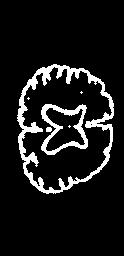
\includegraphics[width=\textwidth, height=\textwidth, trim=0 20 0 20, clip=true, angle=90 ]{figures/diff/bsiBoundary_z.jpg}
        \end{subfigure}
        \caption{BSI boundary region for an AD patient}\label{fig:bsiBoundary}
\end{figure}

\begin{figure}[H]
 \centering
 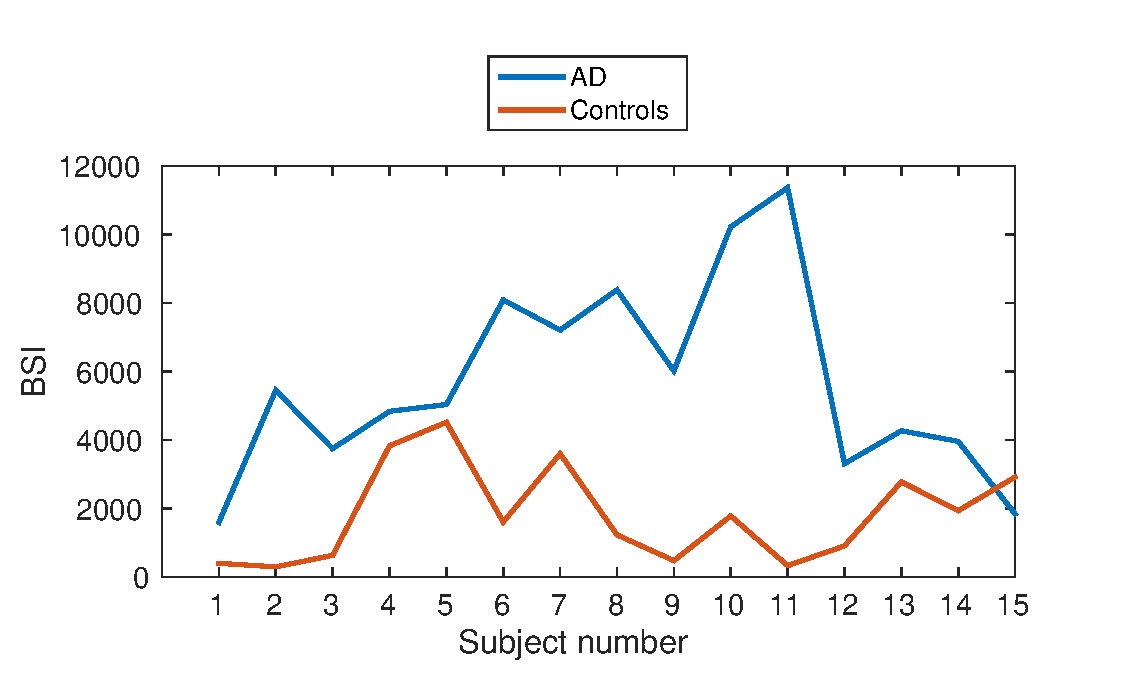
\includegraphics[scale=0.7]{figures/bsi_plot.eps}
 \caption{BSI measurements for all AD and control subjects. Each AD patient is paired with an age-matched control, typically a spouse or carer. \cite{malone2013miriad} There is visibly more atrophy (as measured by BSI) for AD subjects compared to control subjects. The only exception is subject 15, which might be an outlier.}
 \label{fig:bsi_plot}
\end{figure}

\begin{figure}[H]
 \centering
 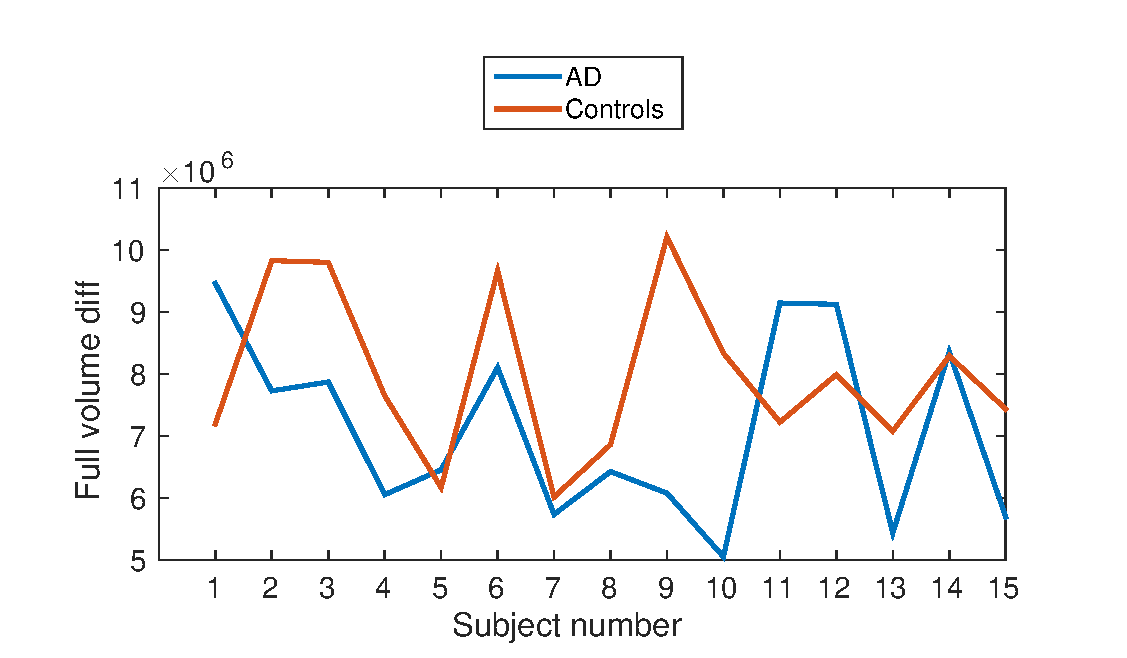
\includegraphics[scale=0.7]{figures/fullVolumePlot.eps}
 \caption{Full volume difference for all AD and control subjects. There is considerable more overlap between AD and control scores compared with the BSI. }
 \label{fig:volumeDiff_plot}
\end{figure}



\section*{Task III - Statistical Analysis}

\subsection*{T-tests}

A two-sample t-test has been performed for AD and control groups using the BSI, in order to see if there is a statistically significant difference in atrophy between AD and control groups (\texttt{p3.m}). Since each AD patient had an age-matched control (normally a spouse or carer ) \cite{malone2013miriad}, this allows us to also perform a paired t-test, checking for a pairwise difference in atrophy. A similar analysis has been made using the full-volume segmentation difference. Results are presented in the following table:\\

\begin{center}
 \begin{tabular}{c | c | c | c | c}
 Metric & \multicolumn{2}{c|}{paired-sample t-test} & \multicolumn{2}{c}{two-sample t-test}\\  
 & $H_0$ & p-value & $H_0$ & p-value\\
 \hline
 BSI & \cellcolor{green!15} rejected & 5.23e-04& \cellcolor{green!15}rejected & 6.45e-05\\
 Seg. volume diff. & \cellcolor{red!15} not rejected & 0.0844 & \cellcolor{red!15} not rejected & 0.1062\\
 \end{tabular}
\end{center}

For the BSI metric, both t-tests rejected the null hypothesis $H_0$, while for the full-volume metric, $H_0$ could not be rejected. We therefore conclude that there is a significant difference of atrophy between AD and control groups, as measured by the BSI. On the other hand, using the full-volume segmentation difference, we conclude that there is no difference between the two groups. This suggests that the BSI is better at discriminating between AD and control subjects than the full-volume segmentation difference. 

\subsection*{Sample size analysis}

MATLAB function \texttt{samplesizepwr} has been used to calculate the sample size required to detect a 25\% atrophy rate with an 80\% power (file \texttt{p3.m}). For the BSI, minimum sample sizes of 34 and 77 are required to detect an atrophy reduction relative to AD and normal ageing respectively. Similarly, for the full segmentation volume difference, minimum sample sizes of 8 and 6 are required to detect an atrophy reduction relative to AD and normal ageing, respectively. The reason for the lower sample size required using the full volume atrophy is because the standard deviation of the groups was much lower relative to the mean.

% sample_size 34, 77, 8, 6


\subsection*{Future improvements}

In order to improve the statistical power of this technique, there are several things one could do:
\begin{itemize}
 \item \textbf{Data acquisition}: Obtain higher-resolution MRI data using 7T (or higher) scanners. In our MIRIAD dataset \cite{malone2013miriad}, a 1.5T scanner was used. 
 \item \textbf{Registration}: A closer look at the registration suggests that there is a lot of room for improvement. We can improve it by calculating the transformation using more iterations at the free-form deformation step. However, other more recent methods such as those based on progressive principal component registration by Melbourne et al. \cite{melbourne2007registration} might obtain better results.
 \item \textbf{Segmentation}: This can be improved by using more templates, or by implementing smarter fusion methods such as weighted majority voting or probabilistic methods such as Non-local-STAPLE or STEPS. One other limitation of this method is that the templates might produce similar labelling errors, but this can be overcome with the method proposed by Wang et al, 2013 \cite{wang2013multi}. One could also combine the segmentation propagation method with other methods based on level sets \cite{cremers2007review}, fuzzy c-means \cite{bezdek1984fcm}, Gaussian mixture models using EM, Markov random fields, Self organising maps \cite{bhandarkar1997multiscale} or Learning vector quantization \cite{karayiannis1999segmentation}.
 \item \textbf{Atrophy estimation}: Perform a bias field correction before BSI computation and do a more robust intensity normalisation and automatic parameter selection based on the intrinsic tissue contrast of the MR images, as described in Leung et al, 2010 \cite{leung2010robust}.
\end{itemize}

Demographic information could also be included in order to improve the statistical analysis. For example, one could compensate for age in the atrophy measurement using the BSI by fitting a linear or polynomial model over the age \& BSI data. The two-sample t-test should show improvements after this change, while the paired t-test shouldn't be affected too much, as the AD and control pairs are already age-matched. If gender information is also available, one could use that to perform a t-test on male and female groups in order to see if the atrophy rate is statistically different. Other demographic information could be used in a similar manner. If multiple types of demographic data is used, one could perform \textit{Canonical Correlation Analysis} in order to find out how much each of these demographic factors are correlated with increased atrophy rate and full volume difference.


\bibliographystyle{unsrt}
\bibliography{citations}

\end{document}





















